\documentclass[final]{beamer}
%\usepackage{mathabx}
\usepackage{arev}

\usepackage{amsmath,amsthm,amssymb,latexsym,bbding}
\everymath{\displaystyle}
\usepackage{mathtools}
% \boldmath

\usepackage[utf8]{inputenc}
\usepackage{csquotes}
\usepackage[english]{babel}
\usepackage[T1]{fontenc}
\usepackage[orientation=portrait,size=custom, height=97,width=97,scale=0.93,debug]{beamerposter}
\mode<presentation>
  {
  \usetheme{IPFposter}
  }


%%%%%%%%%%%%%%%%%%%%%%%%%%%%%%%%%%%%%%%%%%%%%%%%%%%%%%%%%%%%%%%%%%%%%%%%%%%%%%
%% definitions for this poster only



%%%%%%%%%%%%%%%%%%%%%%%%%%%%%%%%%%%%%%%%%%%%%%%%%%%%%%%%%%%%%%%%%%%%%%%%%%%%%%
%% biblatex

\usepackage[backend=biber,citestyle=numeric-comp,bibstyle=BIBStyle,%
            sorting=none,doi=false,hyperref=false]{biblatex}
\bibliography{thebib}
\setbeamertemplate{bibliography item}[text]  % set bibliography item, to show 
                                             % the text of the item (as it 
                                             % comes from biblatex);
                                             % otherwise we get these little 
                                             % images



%%%%%%%%%%%%%%%%%%%%%%%%%%%%%%%%%%%%%%%%%%%%%%%%%%%%%%%%%%%%%%%%%%%%%%%%%%%%%%
%% length and layout fig

\newlength{\columnheight}
\setlength{\columnheight}{97cm}

\setlength\textwidth{\paperwidth}

\newlength{\marginw}
\setlength{\marginw}{2cm}

\newlength{\tw}
\setlength{\tw}{\textwidth}
\addtolength{\tw}{-2\marginw}


\newlength{\colsep}
\setlength{\colsep}{2cm}

\newlength{\colw}
\setlength{\colw}{0.5\tw}
\addtolength{\colw}{-\colsep}


\setlength{\parindent}{0pt}

\setbeamersize{text margin left=0pt,%
text margin right=0pt,%
%sidebar width left=0pt,%
%sidebar width right=0pt,%
%description width=0pt,%
%description width of=0pt,%
%mini frame size=0pt,%
%mini frame offset=0pt%
}

\newenvironment{myTwoColPoster}{%
  \begin{minipage}[t]{\textwidth}%
    \hspace*{\marginw}%
    \hspace*{9.5bp}%  %% dirty trick!!!!
    %\hfill%
    \begin{minipage}[t]{\tw}}%
  {\end{minipage}%
   \hspace*{\marginw}%
   %\hfill%
   \end{minipage}}

\newenvironment{myCol}%
    {\begin{minipage}[t][\columnheight][t]{\colw}}%
    {\end{minipage}}

\newenvironment{textblock}[1]%
    {\begin{block}{\rule[-0.6ex]{0pt}{2.4ex}\raisebox{-0.25ex}[1.6ex]{#1}}%
     \vspace*{5mm}}%
    {\vspace*{5mm}\end{block}}


%%%------------------------------------------------------------------------%%%
%% the document
%%--------------------------------------------------------------------------%%

%% logos
\logoleft{
\includegraphics[keepaspectratio=true,width=9cm]{fig/logos/dd1_1.pdf}}
\logoright{
\includegraphics[keepaspectratio=true,width=9cm]{fig/logos/dd1_2.pdf}}

%% title
  \title[Fraktal Poster4]{{\huge Fraktale Dimensionen}}
  \author[]{\Large Martin Wengenmayr\inst{1,2} \and Ron Dockhorn\inst{1}
    \and Dirk Romeis\inst{1} \and Jens-Uwe Sommer\inst{1,2}} \institute[IPFdd UBS]{ \inst{1}Leibniz-Institut f\"ur
    Polymerforschung Dresden e. V., Hohe Stra\ss e
    6, 01069 Dresden\\
    \inst{2}TU Dresden, Intitut für Theoretische Physik, 01062 Dresden\\
    ~\vspace{1ex} } \date{}

%% set text in footline
\footlinetext{\texttt{http://www.ipfdd.de}\hfill\texttt{wengenmayr@ipfdd.de, dockhorn@ipfdd.de, romeis@ipfdd.de}}


%% replace altert{xx} command :
 %  "(\ \textcolor{IPFred}{.*?} )"  -->  " $1 "

%%--------------------------------------------------------------------------%%
%% content
\begin{document}
\begin{frame}[t]{}
\begin{myTwoColPoster}
% ---------------------------------------------------------%
% first column
\begin{myCol}
  \begin{textblock}{Was ist die Dimension?}
    \renewcommand{\baselinestretch}{1.4}

    {\large \textbf{  \textcolor{IPFred}{Intuitiv} } ist klar welche Dimension $D$ ein \textit{einfaches} geometrisches Objekt besitzt}\\
    \begin{center}
      \hspace*{-1.5cm}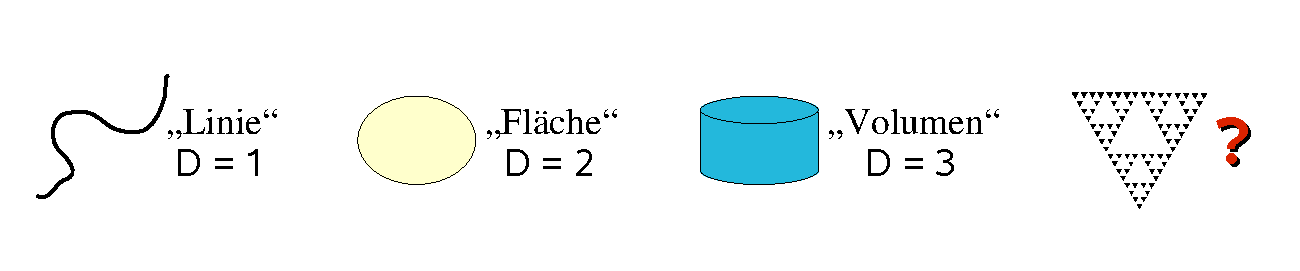
\includegraphics[width=0.8\textwidth]{fig/bsp}\vspace*{-1.5cm}
    \end{center}
    \begin{center}
      \textit{ Gr\"o\ss e} eines Objektes nur sinnvoll definiert im Bezug auf seine Dimension $D$\\
      $\boldsymbol{\Rightarrow}$ Unsinnig zu fragen welche \textit{L\"ange} eine Kugel oder welches \textit{Volumen} ein Rechteck hat
    \end{center}\vspace*{0.6cm}
    {\large \textbf{  \textcolor{IPFred}{Mathematisch} } muss die Dimension $D$ eindeutig formuliert werden}\vspace*{0cm}\\
    \begin{center}
      \begin{itemize}
        \item Ausgangsfrage: Wie gro{\ss} ist die Dimension des Raumes, den das Objekt ausf\"ullt ? 
        \item typische lineare Ausdehnung $r$ : Abmessung in einer Richtung\\
      \end{itemize}\vspace*{0.4cm}
      $\Rightarrow$ \textit{ Gr\"o\ss e} eines Kreises $\sim r^2$\hspace*{1.5cm}\textit{ Gr\"o\ss e} einer Kugel $\sim r^3$\hspace*{1.5cm} \textcolor{IPFred}{Allgemein $\sim r^D$} \\\vspace*{0.8cm}
      \textbf{  \textcolor{IPFred}{Idee:} }Wie viele Kopien $N$ braucht man, f\"ur doppelte Gr\"o\ss e $G\,$?\\
      $\Rightarrow$ $G\to2\,G$\hspace*{1.5cm}durch\hspace*{1.5cm}$N=2^D$ Kopien
    \end{center}
    \vspace*{-1.0cm}
    \begin{center}
    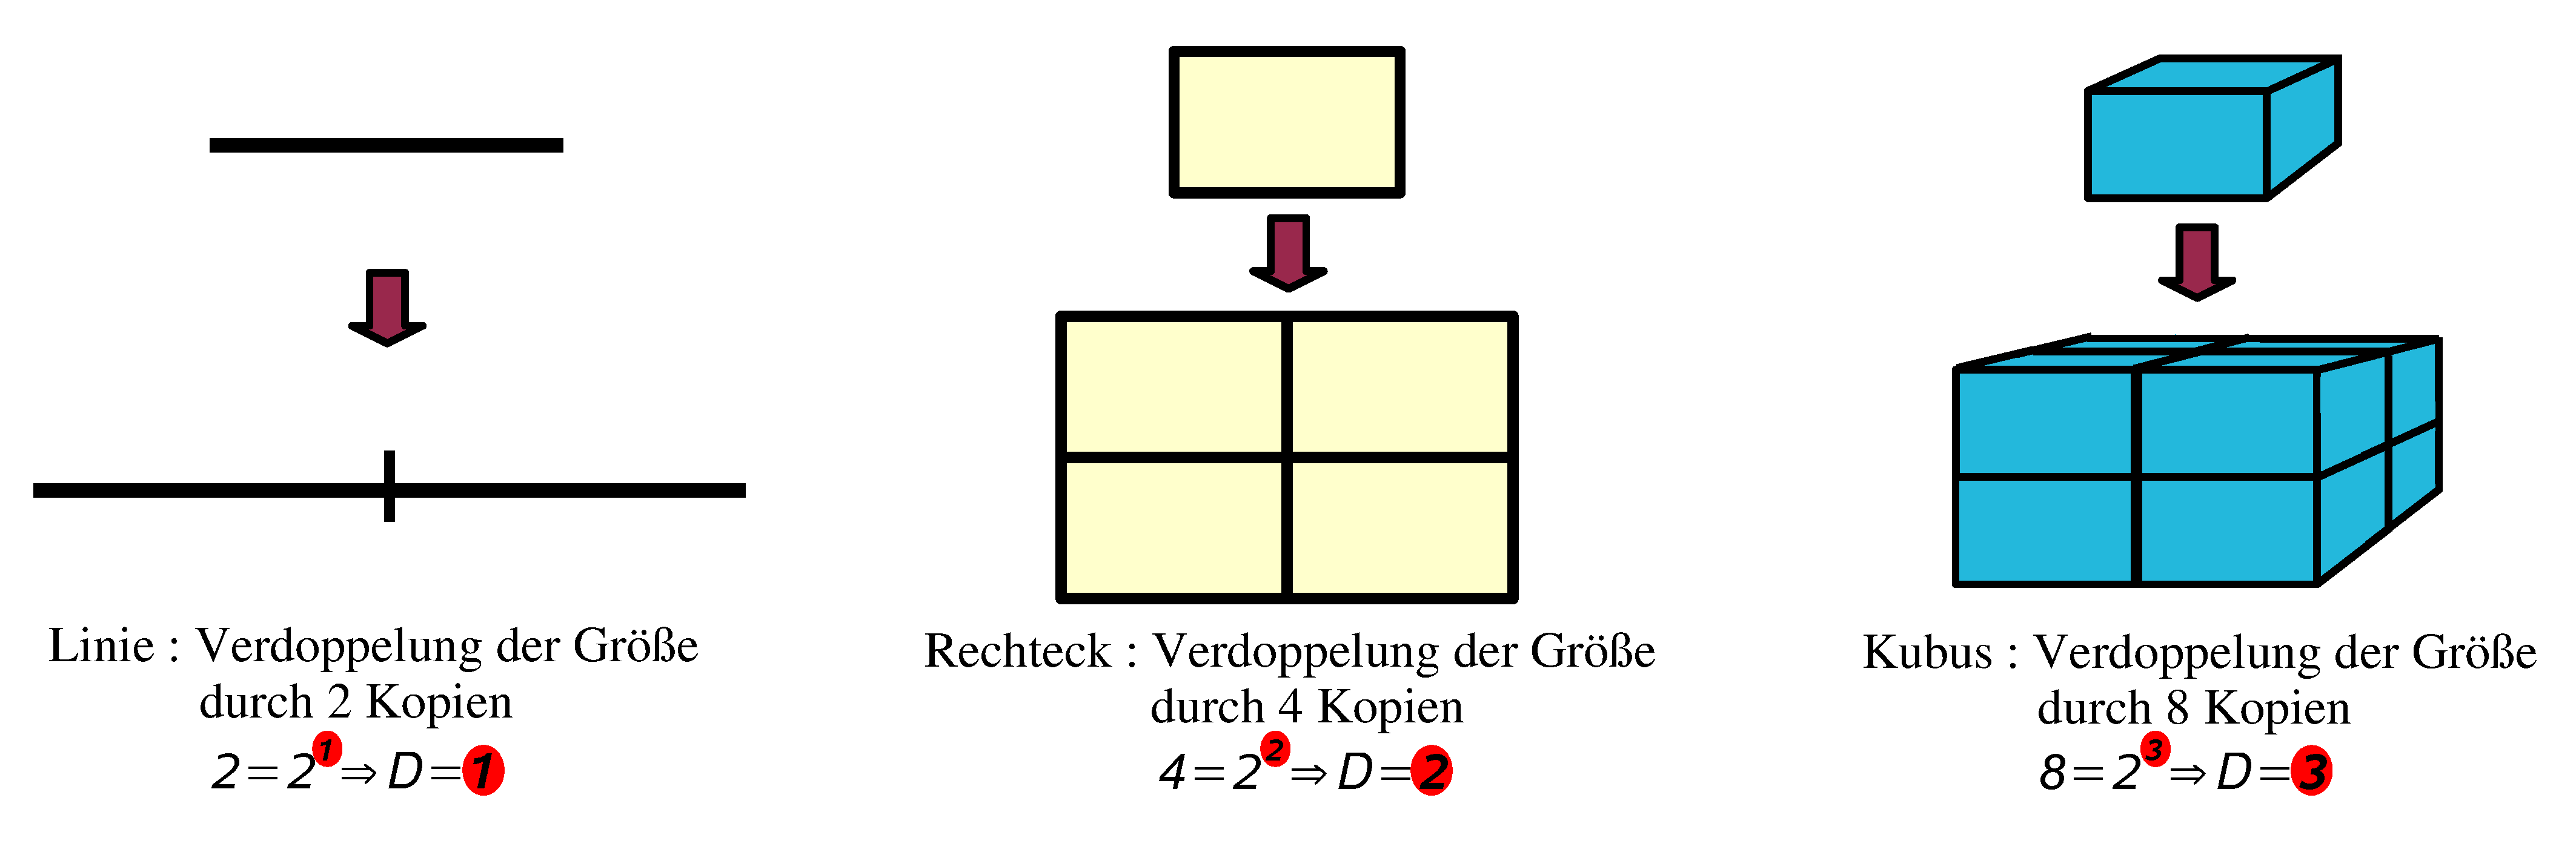
\includegraphics[width=0.8\textwidth]{fig/natD}\\
    \begin{minipage}[c]{0.2\textwidth}
      \centerline{  \textcolor{IPFred}{Allgemein} }
      \centerline{  \textcolor{IPFred}{Hausdorff Dimension} }
    \end{minipage}
    \hspace*{1cm}
    \begin{minipage}[c]{0.01\textwidth}\vspace*{-0.5cm}
      {\LARGE :}
    \end{minipage}
    \begin{minipage}[c]{0.5\textwidth}
      \begin{center}
        F\"ur die $n$-fache Vergr\"o\ss erung des Objekts:\\
        $\boldsymbol{G\to n\,G}$ ben\"otigt man $\boldsymbol{N=n^D}$ Kopien
      \end{center}
    \end{minipage}
  \end{center}

  \end{textblock}
  %%--------------------------------------------------------------------------%%

  

\end{myCol}
% ---------------------------------------------------------%
% end the column
% \hspace*{\colsep}%
\hfill
% ---------------------------------------------------------%
% second column
\begin{myCol}
  
%%--------------------------------------------------------------------------%%

  \begin{textblock}{Fraktale Dimensionen}
  \begin{itemize}
    \item F\"ur kompliziertere oder allgemeinere Objekte ist diese Definition von $D$ sehr n\"utzlich
    \item Verallgemeinerung des Begriffs Dimension auf\,  \textcolor{IPFred}{nicht-ganzzahlige} \,Werte
  \end{itemize}
  \centerline{Aus   \textcolor{IPFred}{$N=n^D$}  folgt, dass   \textcolor{IPFred}{$\ln N=D\,\ln n$}  und somit   \textcolor{IPFred}{$D=\frac{\ln N} {\ln n}$}, also}\vspace*{-0.3cm}
    {\large
      \begin{align*}
        \color{IPFred} D \sim \frac{\ln N(n)} {\ln n}
      \end{align*}
    }
  \begin{minipage}[c]{0.22\textwidth}
    \centerline{ \textbf{ Koch-Kurve}}\vspace*{2.5cm}
    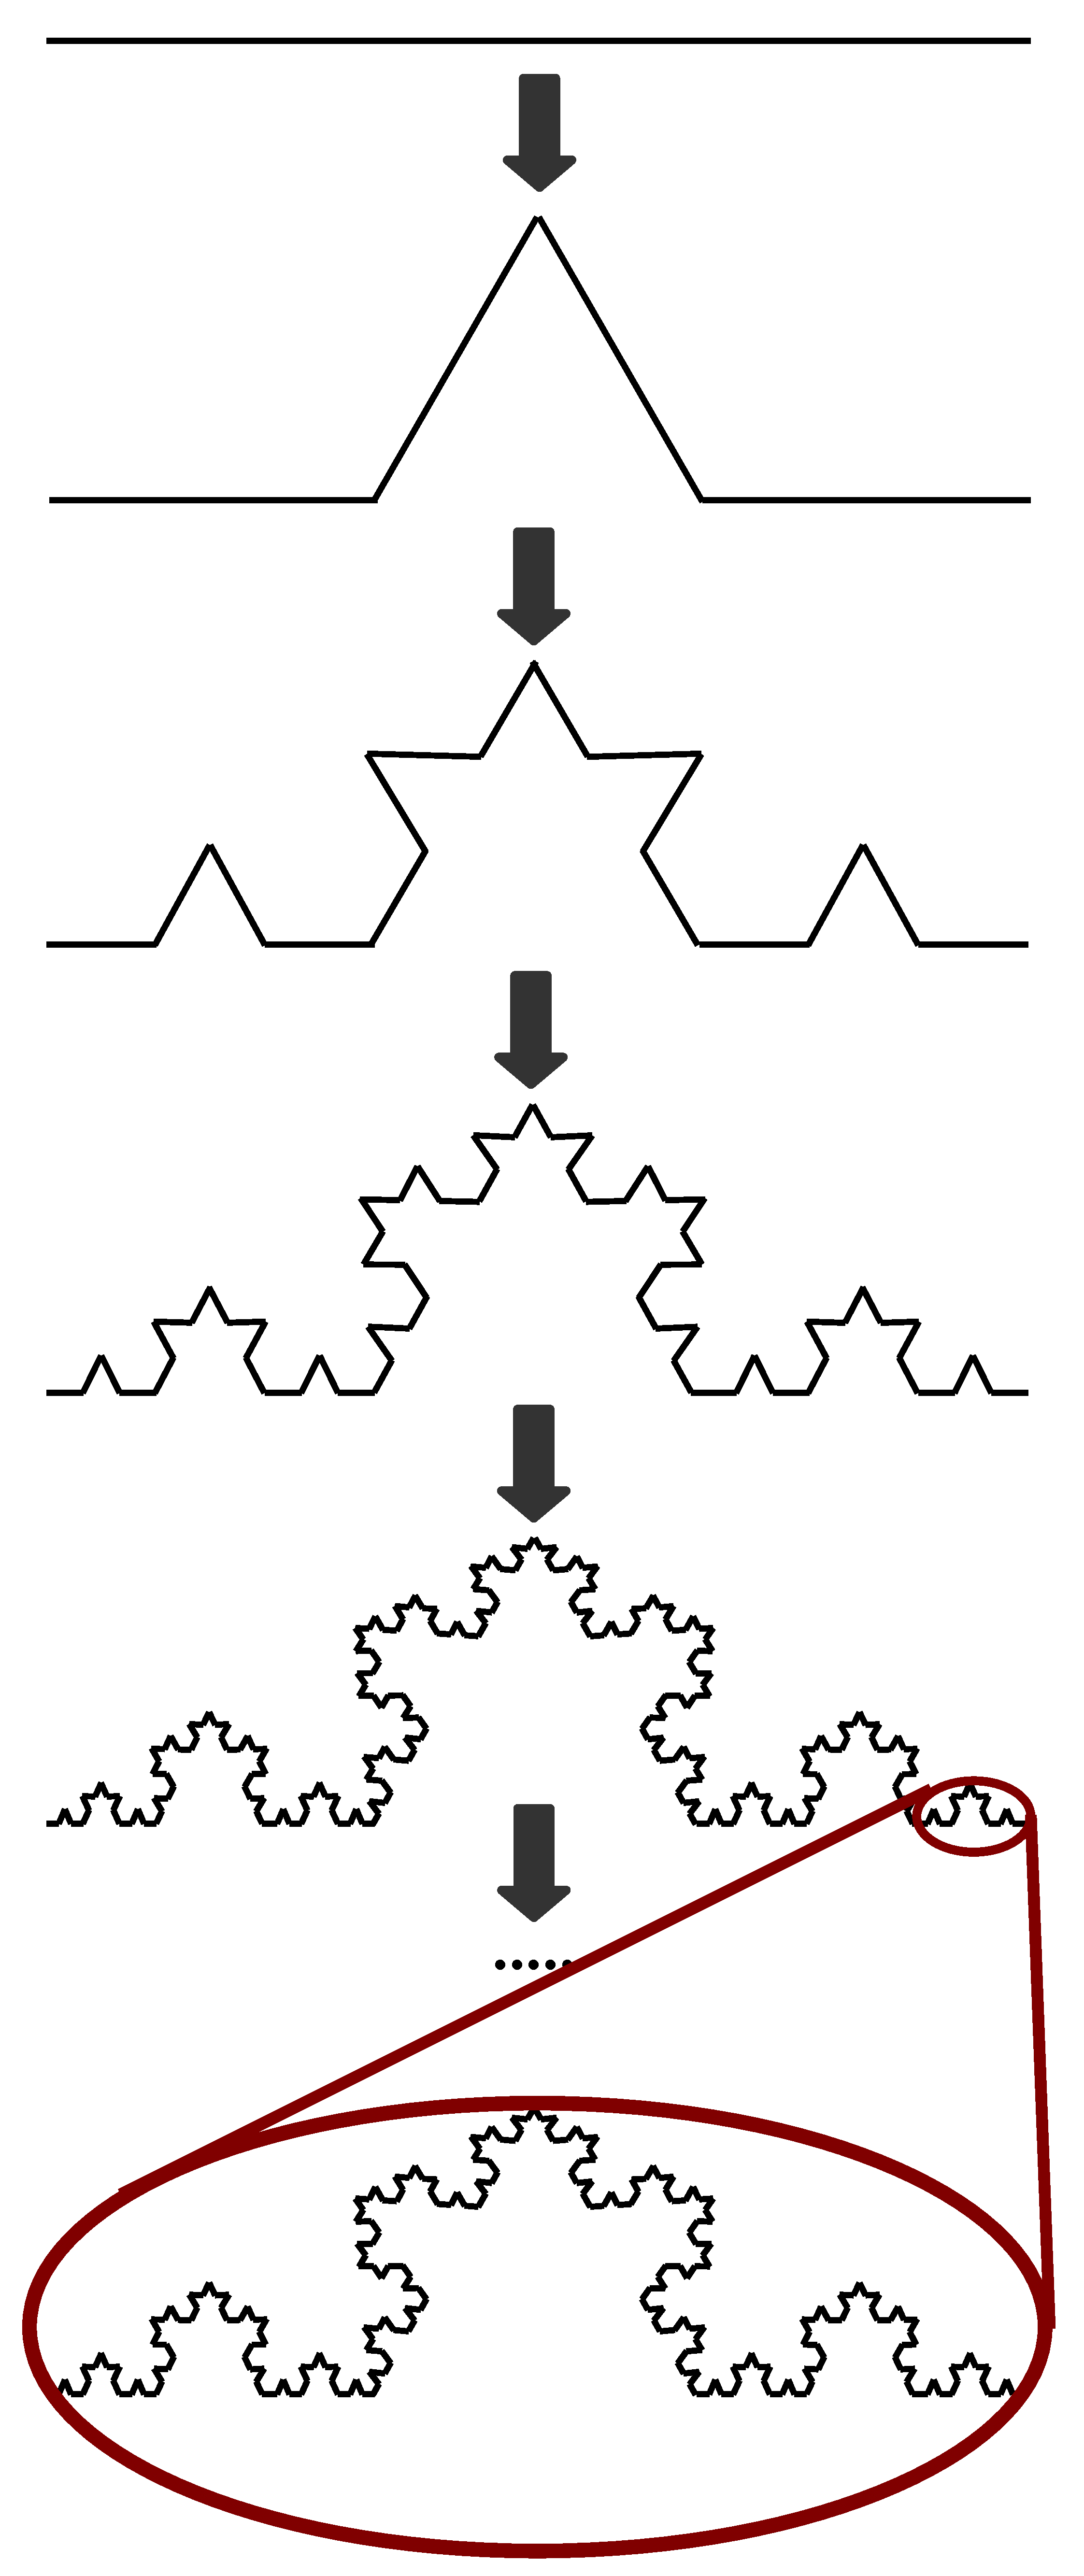
\includegraphics[width=0.99\textwidth]{fig/Koch3}
  \end{minipage}
  \begin{minipage}[c]{0.29\textwidth}
    \centering
    \textbf{ Konstruktion:}\\\vspace*{0.5cm}{\normalsize
    Schneide mittleres Drittel einer Linie aus und setze daf\"ur 2 solcher St\"ucke zu einem Zacken zusammen (immer wieder $\to\infty$)\\
      \textcolor{IPFred}{$\Rightarrow$} Da nach jedem Schritt die Kurve um Faktor $\frac{ 4}{ 3}$ l\"anger wird ist sie am Ende unendlich lang, bleibt aber auf 
    gleiche Fl\"ache beschr\"ankt\\
    \textcolor{IPFred}{\textbf{ Zoomen}} zeigt immer gleiche Struktur
      \textcolor{IPFred}{\textbf{$\Rightarrow$}} Objekt ist \textcolor{IPFred}{\textbf{ selbst\"ahnlich}}  \textcolor{IPFred}{\textbf{ !} } \\
      \textcolor{IPFred}{\textbf{ ?} }$1\leq D\leq2$, aber $D=...$  \textcolor{IPFred}{\textbf{ ?} }\\\vspace*{0.3cm}
    Man kann die Gr\"o\ss e der Koch-Kurve ver-  \textcolor{IPFred}{drei} -fachen indem man  \textcolor{IPFred}{vier} Kopien konstruiert\\
      \textcolor{IPFred}{\textbf{$\Rightarrow$}}   $\textcolor{IPFred}{D} =\frac{\ln 4}{\ln 3}\approx  \textcolor{IPFred}{1,26} $
    }
  \end{minipage}\hspace*{0.7cm}
  \begin{minipage}[c]{0.29\textwidth}
    \centering
    \textbf{ Konstruktion:}\\\vspace*{0.5cm}{\normalsize
    Schneide aus einem Dreieck (schwarz) das zentrale, viertelst so gro\ss e, Dreieck aus und wieder aus den entstehenden schwarzen Dreiecken das zentrale (immer wieder)\\
      \textcolor{IPFred}{$\Rightarrow$} Am Ende hat man einen \textcolor{IPFred}{selbst\"ahnlichen}\textit{ Flickenteppich}\\
    Jeder Schritt hat Fl\"ache um Faktor $\frac{ 3}{ 4}$ reduziert\\\vspace*{0.1cm}
      \textcolor{IPFred}{\textbf{$\Rightarrow$}}  \textcolor{IPFred}{\textbf{ !} }Seine Fl\"ache wird  \textcolor{IPFred}{\textbf{ null} }\\und deshalb muss $D<2$ sein  \textcolor{IPFred}{\textbf{ !} }\\\vspace*{0.3cm}
    Man kann die Gr\"o\ss e des Sierpinski-Dreiecks ver-  \textcolor{IPFred}{zwei} -fachen indem man  \textcolor{IPFred}{drei} Kopien konstruiert\\
      \textcolor{IPFred}{\textbf{$\Rightarrow$}} $  \textcolor{IPFred}{D} =\frac{\ln 3}{\ln 2}\approx  \textcolor{IPFred}{1,58} $\vspace*{0cm}
    }
    \end{minipage}\hspace*{-2.2cm}
    \begin{minipage}[c]{0.21\textwidth}\vspace*{-6.5cm}
    \centerline{\textbf{ Sierpinski-Dreieck}}\vspace*{1cm}\hspace*{1.6cm}
    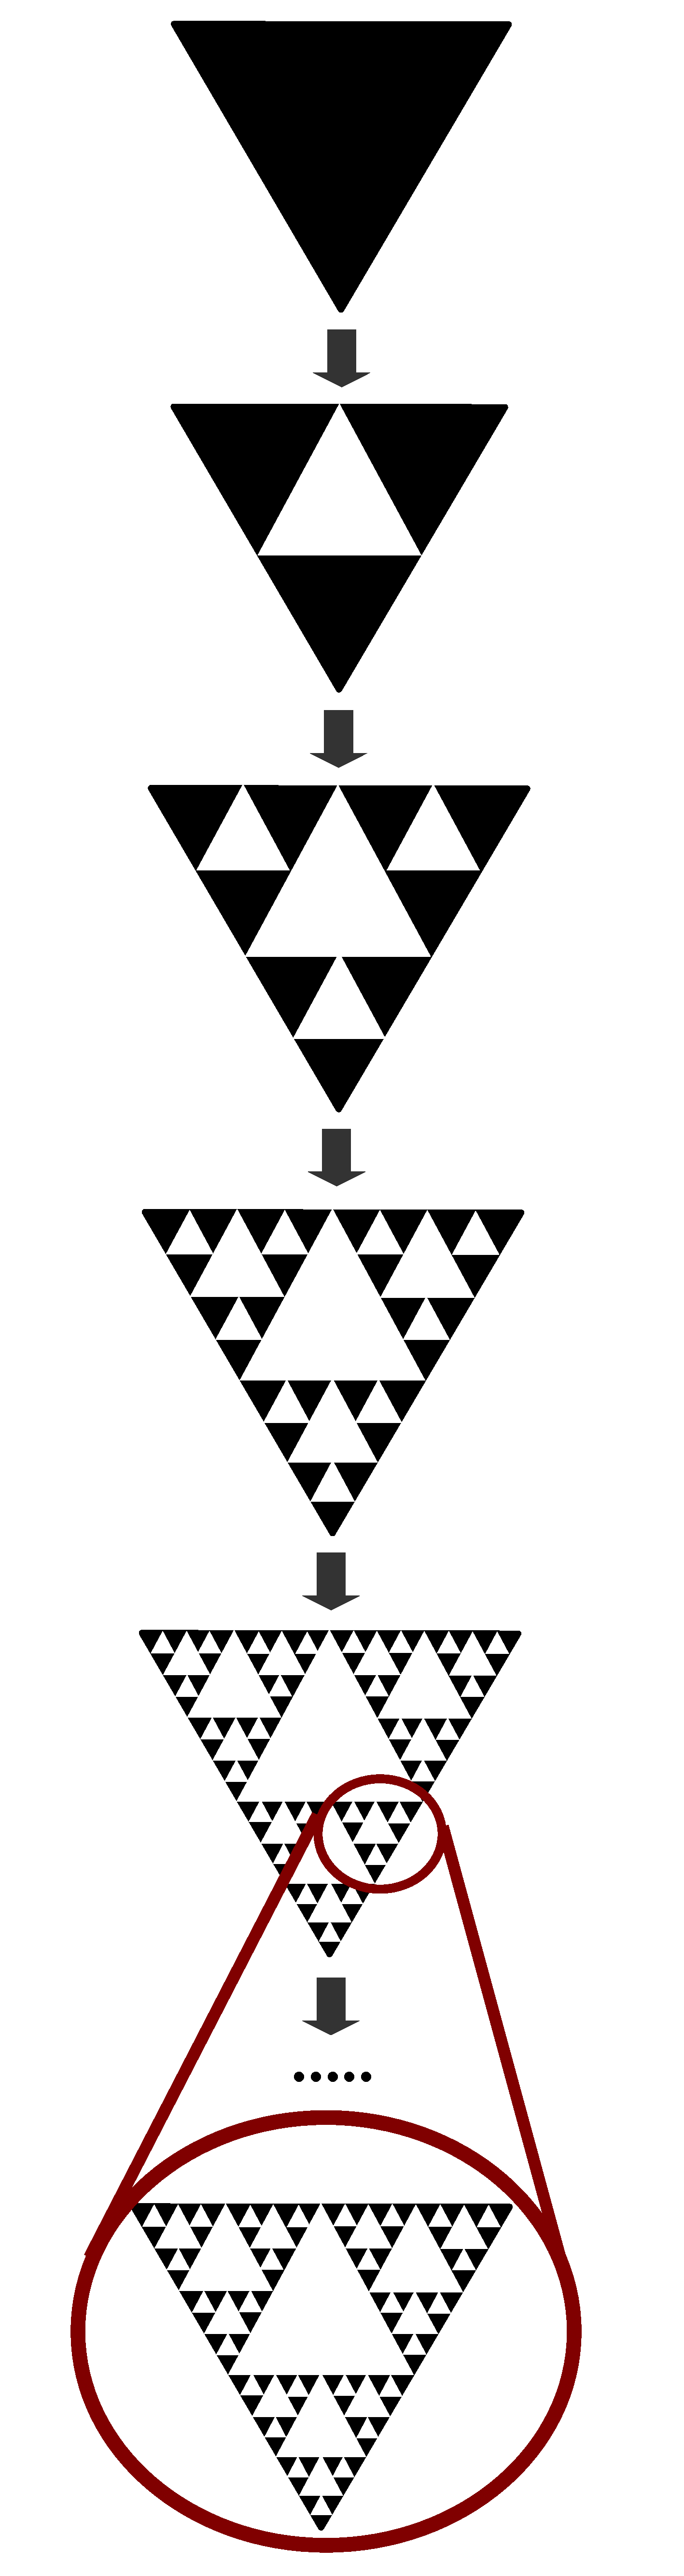
\includegraphics[width=0.48\textwidth]{fig/sierpinski2}
  \end{minipage}
  %\end{center}

\end{textblock}
  %%--------------------------------------------------------------------------%%
  %%--------------------------------------------------------------------------%%


\end{myCol}%
\end{myTwoColPoster}
\end{frame}
\end{document}


%%% Local Variables:
%%% compile-command: "rake makepdf"
%%% End: